\documentclass{article}

\usepackage[printqrbox=false,printhint=true,printanswer=true,printmarkingguide=false]{unswalgos}

\usepackage{tikz}
\usetikzlibrary{patterns}
\usetikzlibrary{shapes,fit}
\usepackage{tkz-fct}
\usepackage{wrapfig}
\usepackage{subfig}

\usepackage{mathtools}
\usepackage{amssymb}
\usepackage{booktabs,multicol,multirow}
\usepackage{wasysym}
\usepackage{tcolorbox}

\DeclareMathOperator*{\argmax}{arg\,max}
\DeclareMathOperator*{\argmin}{arg\,min}
\DeclareMathOperator{\NAND}{NAND}
\DeclareMathOperator{\AND}{AND}
\DeclareMathOperator{\OR}{OR}
\DeclareMathOperator{\NOT}{NOT}

\usepackage{xspace}

\fancyfoot[L]{\leftmark}
\fancyfoot[R]{\rightmark}

% This enables new paragraphs without indentation
\usepackage[parfill]{parskip}

\newcommand{\sem}{23T2}
\newcommand{\semester}{Term 2, 2023}
\SubjectNo{COMP3121/9101}
\newcommand{\taskname}{Assignment 2, Question 2}
\Institution{Algo Rhythm, z1234567} % Replace this with your name and zID


\begin{document}

\setcounter{question}{1}

\begin{Question}

Sam has recently acquired Friendbook, a large social media conglomerate, under dubious circumstances. Since their position as the company's CEO is only probational, they wish to curry favour with the employees by providing raises. However, they don't want to give raises to those who aren't well-known in the company (that would be a waste), and they can't give raises to those who are too well-known (that would raise suspicions). As such, they want to figure out the largest number of people in the company they can give a raise to, without wasting money, and without being caught.

Thankfully for Sam, the company keeps an absurd amount of data on its employees, so they have access to an undirected graph \(G\) of all \(n\) company employees and who they know within the company. In particular, this graph is provided as an \textbf{adjacency matrix} \(M\) such that \(M[i, j] = 1\) if and only if employee \(i\) and \(j\) know each other. An \textbf{induced subgraph} \(H\) of \(G\) is a graph formed from a subset of the vertices of \(G\), where pairs of vertices in \(H\) are adjacent if and only if the corresponding vertices are adjacent in \(G\). In other words, an induced subgraph is formed by deleting some (or maybe none) of the vertices of \(G\), and all adjacent edges.

Sam wishes to find the largest possible induced subgraph \(H\) of \(G\) such that every vertex in \(H\) is adjacent to at least \(k\) other vertices of \(H\), but is also \textbf{not} adjacent to at least \(k\) other vertices of \(H\). Such a subgraph is called ``maximally nepotistic''.

\begin{Subquestion} \label{q:nepo-graph-expl} \textbf{[2 marks]}
    Consider the following graph \(G\) of company connections:
    \begin{center}
        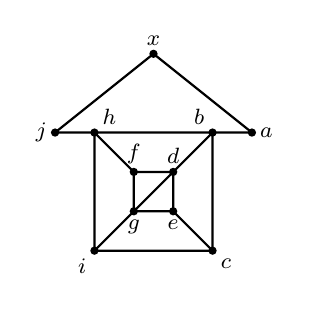
\begin{tikzpicture}[scale=0.5,rotate=-90]
            \foreach \x/\y/\n/\p in {
                0/0/f/above,%
                0/1/d/above,%
                1/0/g/below,%
                1/1/e/below,%
                -1/-1/h/above right,%
                -1/2/b/above left,%
                2/-1/i/below left,%
                2/2/c/below right,%
                -1/3/a/right,%
                -1/-2/j/left,%
                -3/0.5/x/above%
            } {
                \coordinate (\n) at (\x, \y);
                \fill[black] (\n) circle (3pt) node[inner sep=3pt,outer sep=0pt,\p] {\footnotesize\(\n\)};
            }
            \draw[thick, line cap=round] (f) -- (h) -- (j) -- (x) -- (a) -- (b) -- (c) -- (i) -- (h) -- (b) -- (d) -- (e) -- (g) -- (f) -- (d) -- (g) -- (i)
                                            (e) -- (c);
        \end{tikzpicture}
    \end{center}
    With \(k = 3\), explain why any maximally nepotistic subgraph of \(G\) \textbf{cannot} include the vertex labelled \(x\).

\begin{answer}
Since in any nepotistic subgraph, we require any vertices must be adjacent to at least 3 vertices, and $x$ only have two neighbors in $G$, and it can not have more than 2 neighbors in any induced subgraph, which make it impossible be in any nepotistic subgraphs.
\end{answer}

\end{Subquestion}

\begin{Subquestion} \textbf{[2 marks]}
Using the graph \(G\) defined in \ref{q:nepo-graph-expl}, and again with \(k = 3\), find a maximally nepotistic subgraph \(H\) of \(G\), and explicitly list the vertices of \(H\).

\begin{answer}
An maximally nepotistic subgraph with $k=3$ in this graph is the graph induced by the vertices: $\{b, c, d, e, f, g, h, i\}$.
\end{answer}

\end{Subquestion}

\begin{Subquestion} \textbf{[16 marks]}
Given a graph \(G\) with \(n\) vertices and adjacency matrix \(M\), and integer \(k \geq 1\), design an algorithm which finds a maximally nepotistic subgraph of \(G\), if it exists, and lists its vertices. If no such subgraph exists, the algorithm should not output anything. Your algorithm must run in time \(O(n^3)\).

\begin{answer}
We can use a greedy algorithm to solve the problem. The algorithm is as below:

\begin{enumerate}[1]
    \item {
        First we calculate the degree of each vertex, and store them in the 
        array $deg$ ($deg[x]$ is the degree of vertex $x$). Let the number of vertices
        in the current graph be $nc$.
    }
    \item {
        We go through the vertex list in the current graph($G$ at beginning), try to find one vertex
        $x$ either with $deg[x] < k$ or with $deg[x] > nc - k$. If no such vertex 
        x exists, the current graph is a maximally nepotistic subgraph, return it as 
        the answer. Otherwise if we found a such vertex $x$, go to the Step 3. 
    }
    \item {
        For the vertex $x$ we found in the last step, delete it and all its 
        adjacent edges from the current graph, and update the $deg$ values of
        $x$'s neighbors, meanwhile we also update $nc = nc - 1$. After this,
        go to Step 2 to research the current graph.
    }
\end{enumerate}

We now prove this algorithm's correctness by prove (1) All the vertices we delete 
in the process can not be in any nepotistic subgraphs. And (2) the graph we get after 
deleting the vertices is a nepotistic subgraph.

First, we use an inductive way to prove that all the vertices we delete 
in the process can not be in any nepotistic subgraphs.

Base Case: For the first vertex $x_1$ we deleted from the graph $G$. It must follow the condition
 that $deg[x_1] < k$ or $deg[x_1] > nc - k$. If $deg[x_1] < k$, from Subproblem $2.1$ we know it can not 
 be in any nepotistic subgraphs(We explained it before). And If $deg[x_1] > nc - k$, since the nepotistic
 graph requires that every vertex should have at least $k$ other vertices that is not its neighbor. which is 
 $deg[x_1]$ should satisfy that $deg[x_1] \le nc - k$, which contradict $deg[x_1] > nc - k$. Thus
 $x_1$ can not be in any nepotistic graph.

Inductive Steps: If we have that the first $t$ vertices we deleted from the graph can not be in any
nepotistic graphs, consider the $t + 1$ th vertex $x$ we delete. For this vertex it also satisfy the condition 
that $deg[x] < k$ or $deg[x] > nc - k$. Thus the proof is same to the base case. 

In this way, we proved that all the vertices we delete 
in the process can not be in any nepotistic subgraphs.

Next, it's easy to explain why the graph we get after 
deleting the vertices is a nepotistic subgraph. Since in the final graph, no vertex
satisfy the conditions $deg[x] < k$ or $deg[x] > nc - k$. which means $k \le deg[x] \le nc - k$, 
it means that it has at least $k$ neighbors in the subgraph and at least $k$ vertices in 
the subgraph is not its neighbor. Thus the graph is a nepotistic subgraph.

Since we proved that all the vertices that are not in the subgraph can not be in any nepotistic subgraphs,
the graph we get is the maximally nepotistic subgraph.

For the time complexity of the algorithm. In the first step we need to calculate each 
vertex's degree, and since the graph is stored in matrix, the time complexity of this part is 
$O(n\times n) = O(n^2)$. And in the second and third step, we need to delete at most $n$ vertices,
in the second step we need $O(n)$ time to find a vertex to delete(since we have stored the degree of each 
vertex before, we just need to scan through the vertex list). And In the third step we also need $O(n)$ time 
to delete a vertex. Thus the overall runtime of the second and third step is also $O(n^2)$. Therefore the total 
runtime of the algorithm is $O(n^2)$, which is also in the bound $O(n^3)$.
\end{answer}

\end{Subquestion}

\end{Question}

\end{document}